\documentclass[tikz,border=2pt]{standalone}
\usepackage{amsmath,amssymb}
\usepackage{pgfplots}
\pgfplotsset{compat=1.18}

\begin{document}
% Level sets of two quadratic forms: x1^2 + 2 x2^2 (positive definite: ellipses, a bowl) and
% x1^2 - x2^2 (indefinite: hyperbolas, a saddle).
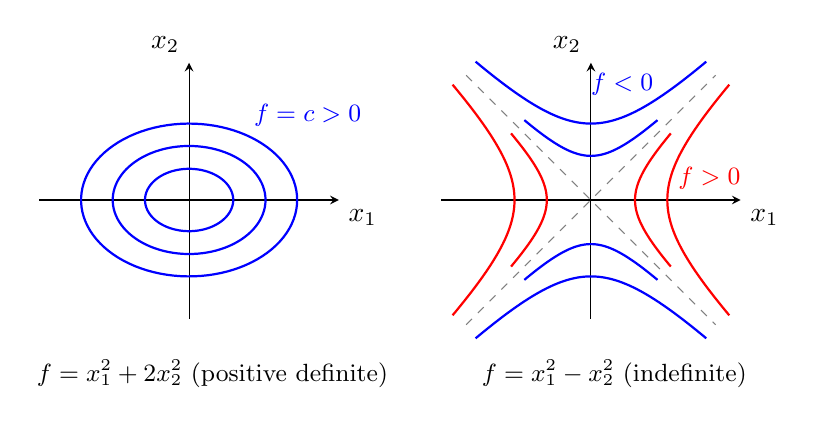
\begin{tikzpicture}
	\begin{axis}[
		name=left,
		axis lines=middle, axis equal image,
		xmin=-2.4, xmax=2.4, ymin=-1.9, ymax=2.2,
		xtick=\empty, ytick=\empty,
		xlabel={$x_1$}, ylabel={$x_2$},
		xlabel style={below right}, ylabel style={above left},
		clip=false, width=5.6cm
		]
		\foreach \c in {0.5,1.5,3} {
			\addplot[blue, thick, domain=0:360, samples=100] ({sqrt(\c)*cos(x)}, {sqrt(\c/2)*sin(x)});
		}
		\node[blue, font=\small] at (axis cs:1.9,1.35) {$f=c>0$};
	\end{axis}
	\begin{axis}[
		name=right, at={(left.east)}, anchor=west, xshift=1.3cm,
		axis lines=middle, axis equal image,
		xmin=-2.4, xmax=2.4, ymin=-1.9, ymax=2.2,
		xtick=\empty, ytick=\empty,
		xlabel={$x_1$}, ylabel={$x_2$},
		xlabel style={below right}, ylabel style={above left},
		samples=100, clip=false, width=5.6cm
		]
		\addplot[gray, dashed, domain=-2:2] {x};
		\addplot[gray, dashed, domain=-2:2] {-x};
		\foreach \c in {0.5,1.5} {
			\addplot[red, thick, domain=-1.2:1.2] ({sqrt(\c)*cosh(x)}, {sqrt(\c)*sinh(x)});
			\addplot[red, thick, domain=-1.2:1.2] ({-sqrt(\c)*cosh(x)}, {sqrt(\c)*sinh(x)});
			\addplot[blue, thick, domain=-1.2:1.2] ({sqrt(\c)*sinh(x)}, {sqrt(\c)*cosh(x)});
			\addplot[blue, thick, domain=-1.2:1.2] ({sqrt(\c)*sinh(x)}, {-sqrt(\c)*cosh(x)});
		}
		\node[red, font=\small] at (axis cs:1.9,0.35) {$f>0$};
		\node[blue, font=\small] at (axis cs:0.5,1.85) {$f<0$};
	\end{axis}
	% Panel titles go below the panels, clear of the x_2 axis labels.
	\coordinate (low) at (current bounding box.south);
	\node[anchor=north, font=\small] at ([yshift=-4pt]left.outer south |- low) {$f=x_1^2+2x_2^2$ (positive definite)};
	\node[anchor=north, font=\small] at ([yshift=-4pt]right.outer south |- low) {$f=x_1^2-x_2^2$ (indefinite)};
\end{tikzpicture}
\end{document}
